\section{NSCs}

Im folgenden die wichtigsten Charaktere mit denen es die Spieler zu tun bekommen aufgeteilt nach Ort des Geschehens.

\subsection{Cowboybrigade}

Die Cowboybrigade sind 5 Alphas, Spezialisten f"ur Raumschifftechnik, Arbeit mit Exoskelett im Luftlehren Raum, Drohneneinsatz.
Angestellt bis vor 6 Wochen am Raumhafen von Valhalla auf Callisto. Dann ausgeliehen an die Protektoratsgarnison am Raumhafen von Valhalla und vor ca.~4 Wochen ausgeliehen an Armageddon. Die Cowboybrigade stammt urspr"nglich aus dem Asteroideng"urtel G"urtel zwischen Mars und Jupiter und ist vor wahrscheinlich einem Jahr auf Callisto.

\begin{itemize}
    \item Stetson: Der Anf"uhrer, gro\3 und dratig.
    \item Quckfinger Rod: Vorlaut, immer ein Kartenspiel in der Hand.
    \item Joe Rider: Klein, gedrungen, spricht nicht wenn nicht unbedingt n"otig.
    \item Tom Gunslinger: Der Vern"unftige.
    \item Slingshot (Drake): Das "`Nesth"akchen"' der Gruppe. Drake ist der Name unter dem er in nach dem Attentat auf Armageddon auf Hellgate auftaucht.
\end{itemize}

Slingshot ist einer der Attent"ater, ein Alpha dessen Gehirn durch eine von der USI kontrollierten KI "ubernommen wurde.
Auf Hellgate tritt er nach dem Vorfall auf Armageddon unter dem Namen Drake auf.

\textbf{Slingshot: Fight +4, Agility +4, Body +2, HP 10}

\newpage

\subsection{Pers"onlichkeiten auf Hellgate}

Auf Hellgate gibt es folgende Pers"onlichkeiten:

\begin{itemize}
    \item Dr.~Acra Link: Technische Leitung der Hellgate Station
    \item Sina Hendrik: Administrative Leitung der Hellgate Station
    \item Dr.~Petrova: Technische Leitung der F"orderminen
    \item Henk Arongate: Sicherheitschef    
    \item Kriegsmeister Jos\'{e} \frqq{}Toro\flqq{} Alvarez: Norm. Ausbilder der Jagdverb"ande des Protektorats, Kriegsheld.
    \item Arbeiter Mob: Fight +2, Agility +1, Body +3, HP 10, Courage +2
\end{itemize}

\subsection{Sicherheitspersonal Hellgate}

Neben \emph{Grace Anders} sind folgende Personen des Sicherheitsdienstes relevant:

\begin{itemize}
    \item Henk Arongate: Sicherheitschef    
    \item Karl Sandos: Stationsleiter des St"utzpunkts der Sicherheitskr"afte. Vorgesetzter von Grace Anders.
    \item Luke Dexter: Trupp F"uhrer der Sondereinsatzgruppe f"ur die Befreiung der Geiseln.
    \item Luke Lengdon: Mitarbeiter Sicherheitsdienst. Wird bei der Geiselname auf dem Sicherheitsst"utzpunkt schwer verletzt. Ehemaliger Freund von Grace Anders. Seit 2 Wochen getrennt.
\end{itemize}

\newpage
\subsection{Grace Anders}

Grace Anders ist eine Mitarbeiterin des Sicherheitsdienstes auf Hellgate. Sie wird von Chef Henk Arongate zur Unterst"utung der Charaktere abgestellt. 

\begin{wrapfigure}{l}
    {0.45\textwidth}\fbox{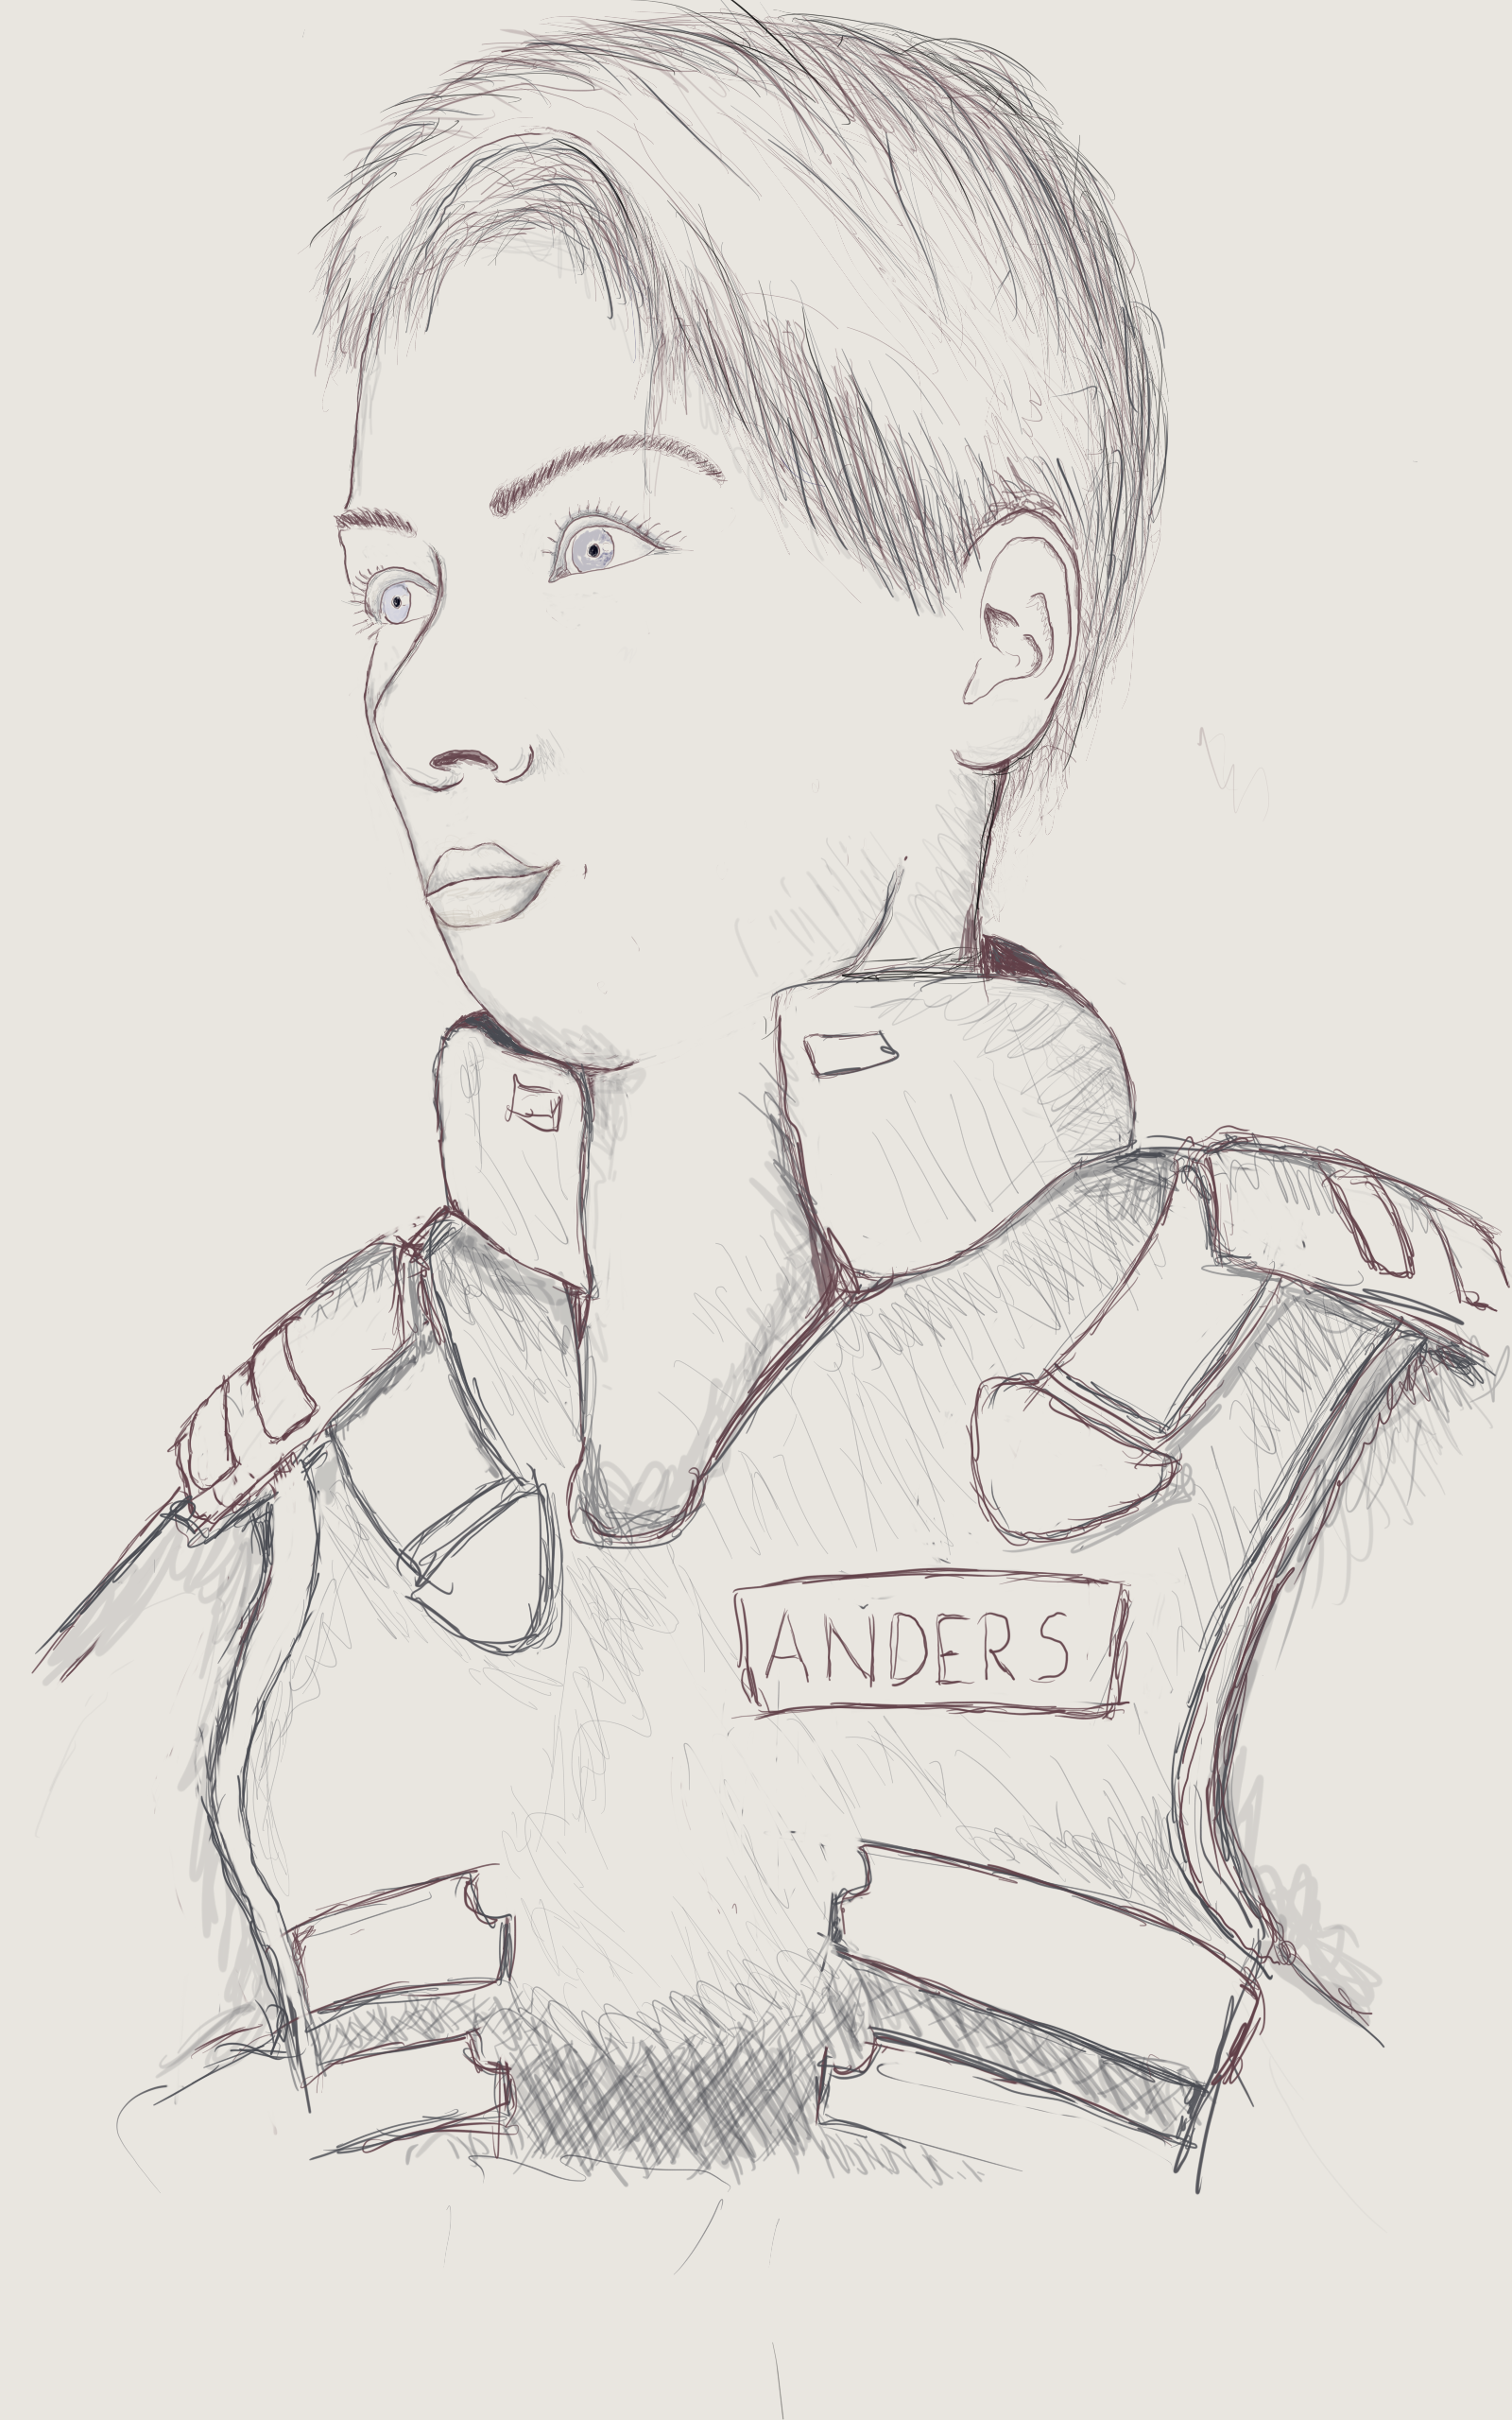
\includegraphics[width=0.90\linewidth]{./images/grace_anders_p.png}}
    \caption{Grace Anders}
\end{wrapfigure}

Grace Anders ist Mitte 30, h"ubsch mit kurzen blonden Haaren. W"ahrend der Unterst"utzung der Charaktere tr"agt sie die Schutzkleidung des Sicherheitsdienstes mit schu\3sicherer Weste, Schlagstock, Handschellen und einer Schu\3waffe. 

Sie stammt urspr"unglich vom Mars und hat sich ins Jovianische System auf der Suche nach neuen Herausforderungen versetzen lassen. Sie war mit Luke Lengdon der Sicherheitsmann bei der folgenden Geiselname schwer verletzt wurde liiert hat sich aber vor kurzem von ihm getrennt.

Die Sicherheitsbeamtin begleitet die Charaketere w"ahrend des aufenthalts auf Hellgate und berichtet regelm"aßig an \emph{Karl Sandos} ihren vorgesetzten. "Uber Grace Anders k"onnen sie Informationen bzgl.~der Minen und Personal der Station und der Mienen anfragen. W"ahrend der Entf"uhrung kann sie die Charaktere unterst"uten.

Grace Anders: Fight +4, Agility +3, Body +2, HP 10

\subsection{Besatzung HeM05}

Folgende Personen waren w"ahrend des Attentats auf HeM05:

\begin{itemize}
    \item Florence: Beta Mutant, Kommandant der Mine    
    \item ZDee: Alpha Mutant Minenarbeiter (tot)
    \item Greydog: Alpha Mutant, Minenarbeiter
    \item Isabell Sonderleiten: Norm, Chemikerin, Stellvertreterin von Florence
    \item Juri Smirnov: Norm, Logistik
    \item Fernandez Lorend: Norm, Techniker
    \item Hanibal: Alpha Mutant, Techniker der Minensteueranlage, Attent"ater
    \item Pitch: Alpha Mutant, Technikerin der HE-3 der Minensteueranlage
    \item Salvador: Norm, Physiker, Weltraumtechnik
    \item Blackwind: Beta, Sicherheitsdienst
\end{itemize}

All Mitarbeiter auf der Mine au\3er Fernand, Salvador, Greydog und Pitch waren vor dem Jupitereinsatz bereits im Dienst der Cynarion Corporation.

\subsection{Commander Lockhead}

Commander Lockhead ist der Kommandant der Milit"argarnison des Protektorats auf Valhalla. Commander Lockhead ist ein Omega Veteran der bereits ein wenig in die Jahre gekommen ist und deshalb f"ur einen Omega sehr umg"anglich ist.


\newpage
\subsection[Wang Xiao Saber Long]{\pinyin{Wang2} \pinyin{Xiao3} \frqq{}Saber\flqq{} \pinyin{Long2}}

\pinyin{Wang2} \pinyin{Xiao3} \frqq{}Saber\flqq{} \pinyin{Long2} entstammt einer reichen Familie aus den F"uhrungsreihen der USI Corporation. Fr"uhzeitig hat sie sich von ihrer Familie abgewandt und hat sich aus Luna abgesetzt um einen Schmugglering f"ur Hilfsg"uter im Asteroideng"urtel zu gr"unden. Ihr Schiff wurde Piraten aufgebracht und sie geriet in Gefangenschaft. Nach der "Ubernahme des Kaperschiffs und Zusammenf"uhrung mit ihrer Schmugglerbande macht sie sich einen Namen als ber"ucktigsten Pirantenf"uhrer des Pirantenverband Roter Drache mit dem Emblem eines schwaren Drachens auf rotem Grund.

\begin{wrapfigure}{r}
    {0.55\textwidth}\fbox{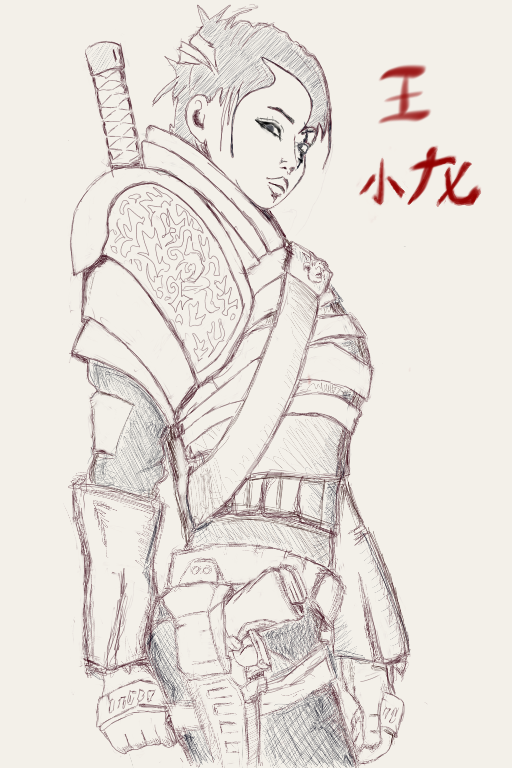
\includegraphics[width=0.9\linewidth]{./images/wang_xiao_long.png}}
    \caption{\pinyin{Wang2} \pinyin{Xiao3} \pinyin{Long2}}
\end{wrapfigure}

Nach ihrer Gefangennahme wurde sie vor zwei Jahren zum Hochsicherheitsgef"angnis Blackpit auf Vahlhalla verlegt. Dort machte man ihr das Angebot einer Haftentlassung im Gegenzug zur Teilnahme an einem klinischen Experiment.

Beim durchgef"uhrten klinischen Experiment handelt es sich um das Einsetzen einer der von Prof.~Dr.~Naratova entwickelten ``freien KI'' Symbionten. Die Oeration wurde durch Prof.~Dr.~Sanders durchgef"uhrt. Prof.~Dr.~Sanders handelte dabei im direkten Auftrag von Prof.~Dr.~Naratovas ohne das Wissen der USI Agenten Smith-Singer und Frederic Johnson. Durch ihre starke Pers"onlichkeit konnte \pinyin{Xiao3} \pinyin{Long2} verhindern da\3 die KI ihren Geist vollst"andig "ubernehmen konnte und so verschmolzen der Geist und das artifizielle Gehirnzu einer Symbiose genau so wie Prof.~Dr.~Naratova es sich immer erhofft hatte.

Nach ihrer Haftentlassung schlo\3 sich \pinyin{Xiao3} \pinyin{Long2} dem Luna--Syndikats untern dem Stra\3ennamen Saber (Stra\3ensamurai) an und stieg dort schnell zu einem der Capos der Organisation auf. Duke Nemessis wei\3 um ihre Vergangenheit. Die Verwandlung in eine KI ist ihm allerdings nicht bekannt. Ihm ist Sie als geflohene Verrecherin bekannt.

\pinyin{Xiao3} \pinyin{Long2} ist eine hochgewachsene Asiatin anfang 40, ein Pure, die sich als Saberurai mit entsprechender R"usting gibt. Sie ist intelligent, gewitzt, skrupellos und liebt das Risiko. Durch ihre finanziellen M"oglichkeiten und Kontakte in ihrem fr"uheren Leben hat Sie ihren K"orper durch zahllose Modifikationen zu einer Kampfmaschiene entwickelt die einem Omega in nichts nachsteht was f"ur einen Norm sehr ungew"ohnlich ist. Ihr Stra\3enname Saber in Valhalla ist an die Bezeichnung Stra\3ensamurai angelehnt.

Im Rahmen des Abenteuers verfolgt sie das Ziel die Forschungsergebnisse Naratovas an sich zu bringen und alle Informationen zu den freien KIs wie auch das Wissen "uber die Technologie zu vernichten. Daf"ur wird sie alle an den Experimenten beteiligten Personen Naratova, Sanders, die USI Agenten und deren Wissenschaftler t"oten und Forschungseinrichtungen zerst"oren solange sie dabei den Verdacht nicht auf sich lenkt. An der Identit"at der anderen KIs ist sie nicht interessiert.

Vor dem Zusammentreffen mit den Charakteren kennt sie den Standort und den Namen der USI Tochter Cyberbrain nicht.

\pinyin{Wang2} \pinyin{Xiao3} \pinyin{Long2}: Fight +9, Agility +10, Body +4, HP 14

\subsection{Carina alias Fleur Soleil}

\begin{wrapfigure}{r}
    {0.50\textwidth}\fbox{
\includegraphics[width=0.9\linewidth]{./images/carina.png}}
    \caption{Carina}
\end{wrapfigure}

Die als geheimnisvolle Freundin von Slingshot erstmals aufgetauchte Frau mit auff"alligen roten Haaren ist im Blackhole Club als Carina bekannt und stellt dort Kontakte zwischen Anbietern und Interesenten von Waren und Dienstleistungen her. Sie arbeitet dabei mit dem Barmann Rosen zusammen. Im Ice Club tritt sie unter dem Namen Fleur Soleil als S"angerin und f"ur ausgew"ahlte Kundschaft auch f"ur andere Dienste auf. Carina ist sehr h"ubsch, vielleicht Ende 20 und lebenslustig. Ihr auff"alligstes Merkmal und Markenzeichen sind lange kunstvoll geflochtene Haare. Die Farbe der Haare kann sie je nach Stimmung und Gelegenheit in nahezu beliebige Farben wechseln.

Carina hat den Erstkontakt von Hanibal und Slingshot zu den USI Agenten Smith--Singer und Frederic Johnson hergestellt. Mit Slingshot war sie f"ur kurze Zeit n"aher befreundet und ist entsprechend von seinem Tod und ihrer Mitt"aterschaft ersch"uttert und will den Ermittlern 
aus diesem Grund auch weiterhelfen.

\subsection{Nemessis}

Nemessis ist der Duke von Valhalla, der Pate des Luna--Syndikats. Nemessis ist ein Slag dessen K"orper sich nicht mehr selbst am Leben erhalten kann. 

\begin{wrapfigure}{r}
    {0.70\textwidth}\fbox{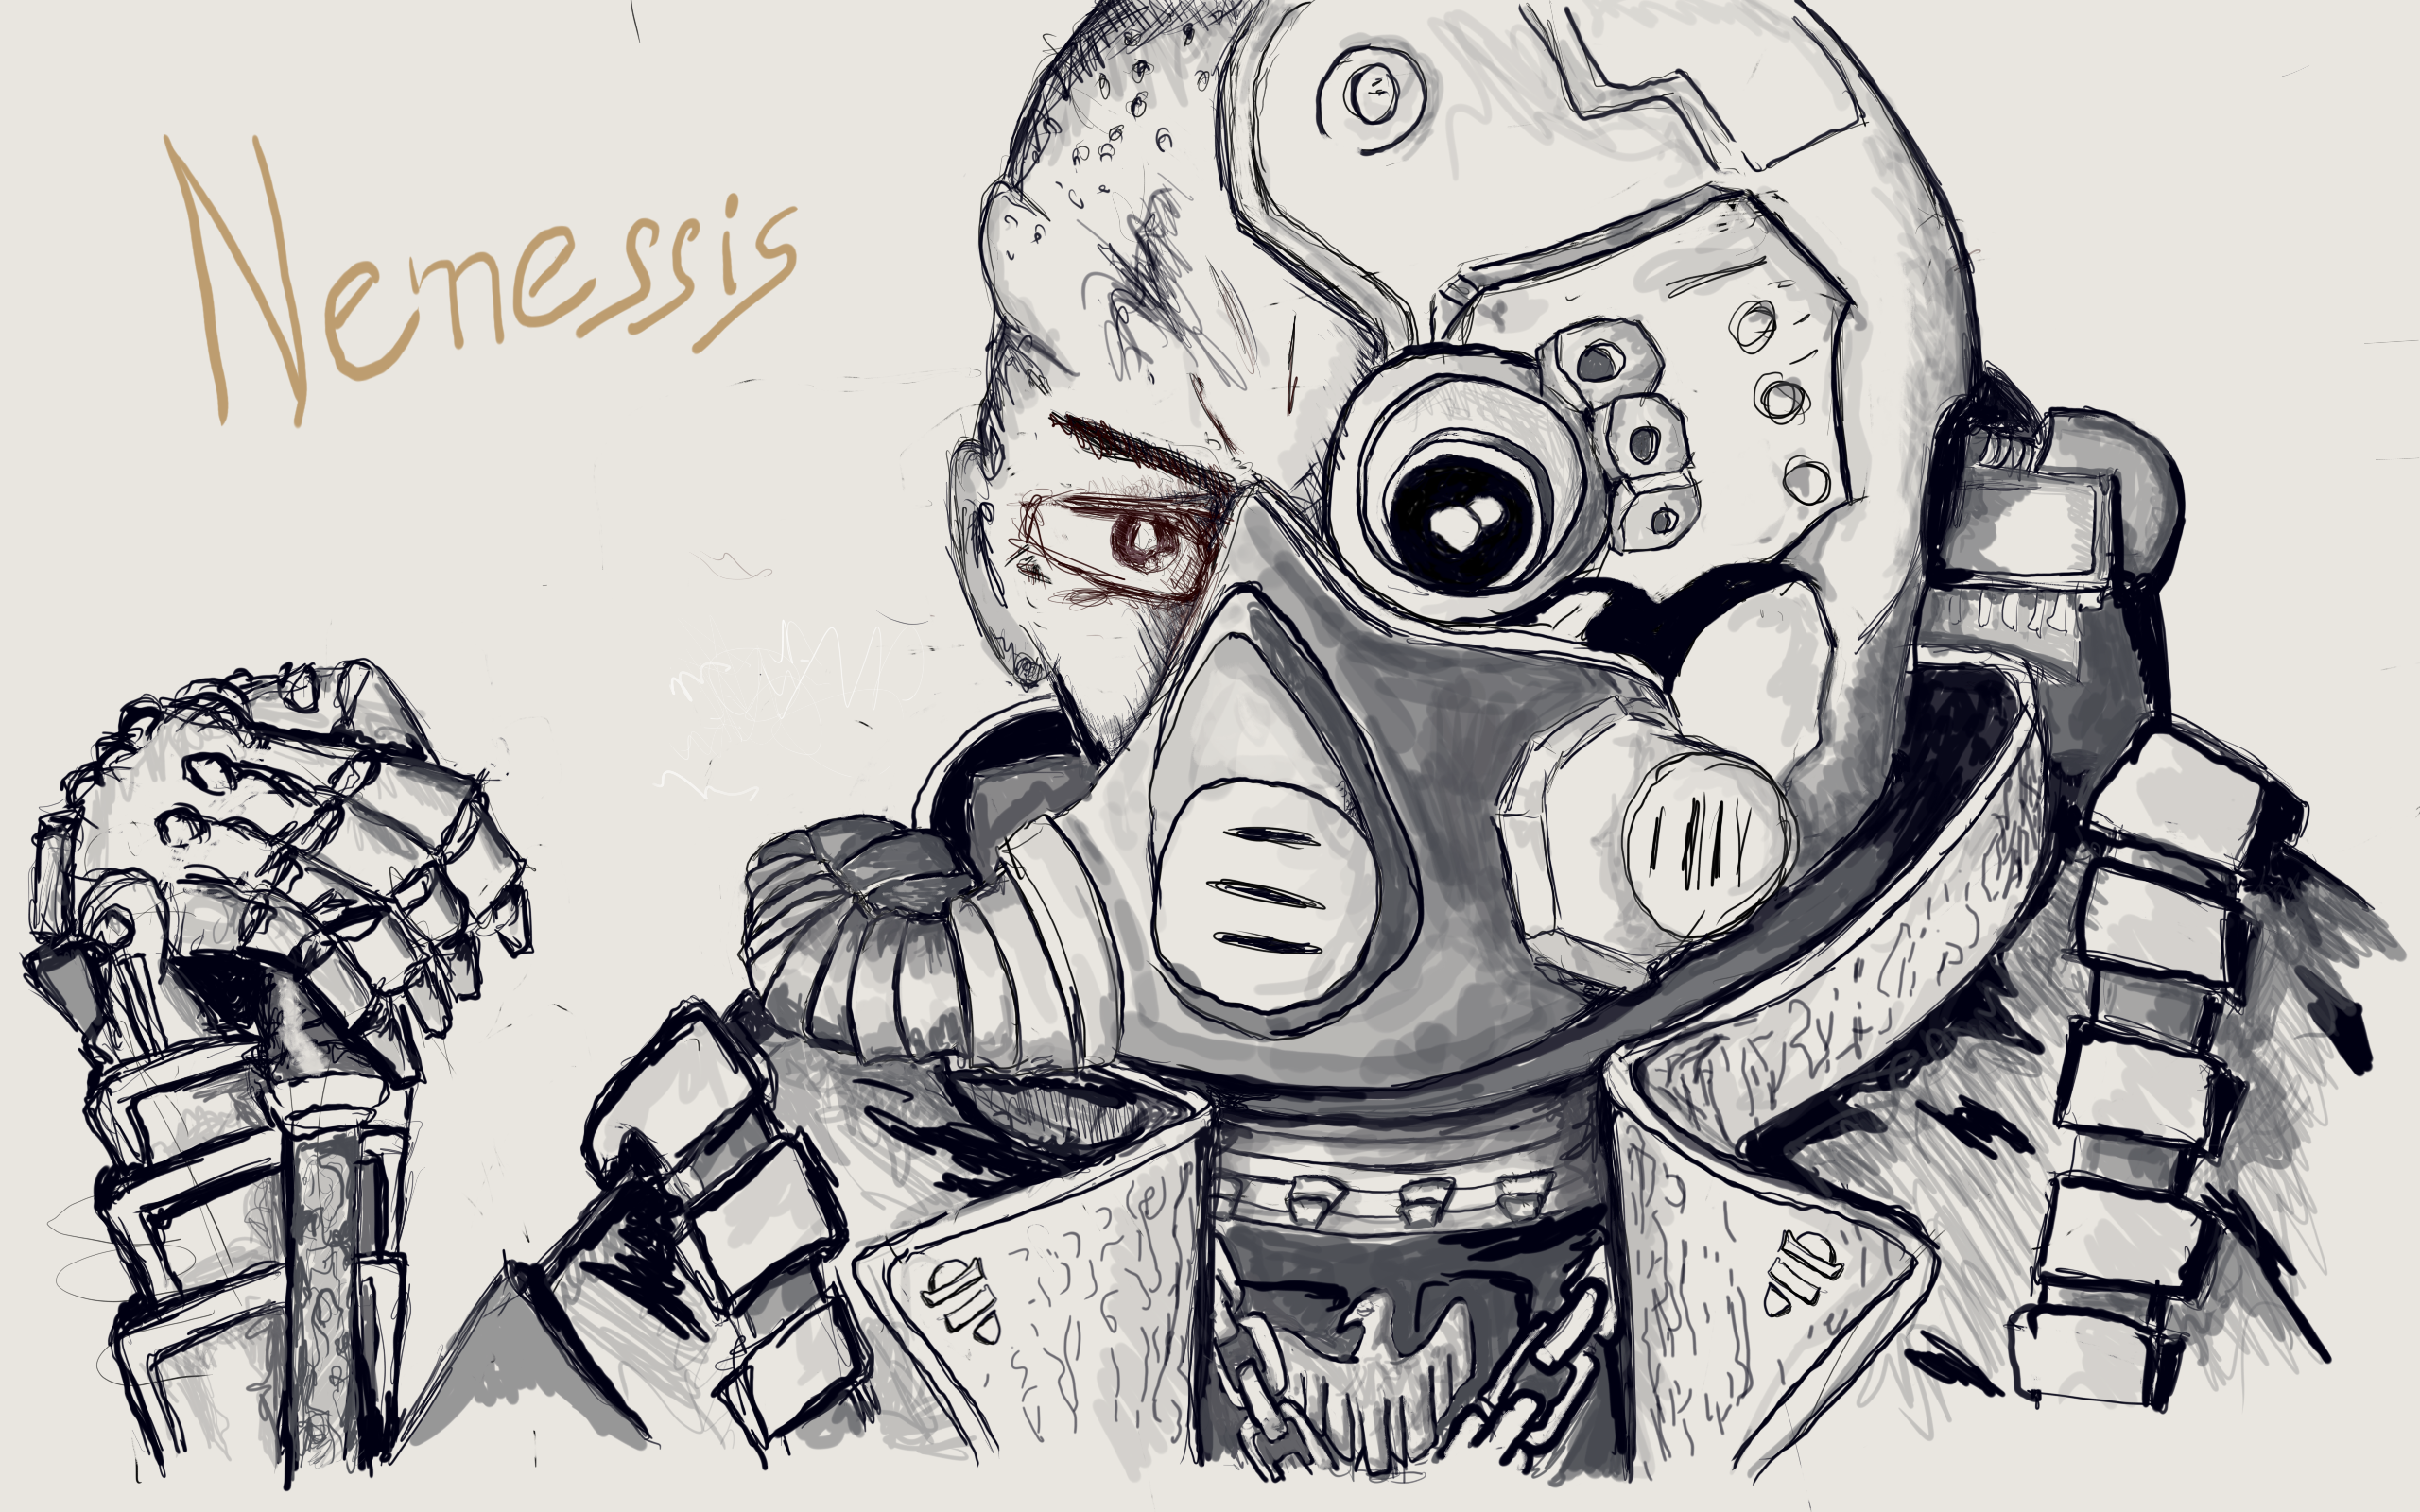
\includegraphics[width=0.9\linewidth]{./images/nemessis.png}}
    \caption{Nemessis}
\end{wrapfigure}

Ein Gro\3teil seiner Gliedma\3en und sonstigen K"orperfunktionen sind durch synthetische Teile ersetzt die Ihm das Aussehen eines Cyborgs geben. Nemessis hat die Unterwelt auf Valhalla durch seine gut organisierten Untergebenen und sein weitreichendes Kontaktenetz
fest im Griff. Das Syndikat betreibt das lokake Fusionskraftwerk von Valhalla und damit die Lebensversorung. Ein Gro\3teil der Etablisments in Paradise City werden vom Luna Syndikat betrieben. Nemessis hat mit Blackheart die Vereinbarung getroffen da\3 sich die Protektoratsstreitkr"afte nicht in seine Aktivit"aten einmischen er daf"ur den reibungslosen Betrieb Valhallas sicherstellt.


\newpage
\subsection{USI Agenten}

Die United Space Industry (USI) finanziert das KI Projekt, betreibt "uber Stohfirmen die Cyberbrain Forschungseinrichtung auf Kallisto und beauftragt die Attent"ater. Vor Ort im jovianischen System koordiniert der Agent \emph{J.~Smith--Singer} die Operation P9. Smith--Singer wird druch den Psychonauten \emph{Frederic Johnson}, den Strohmann \emph{Bloe Ringdan} und die beiden S"oldner \emph{Lazor} und \emph{Flinn}. Den Erstkontakt zu Prof.~Dr.~Naratove stellte ein Agent her den der Ermittlercharakter als Prolog Interviewen durfte.

Smith--Singer gibt sich als Agent des Konzernrat aus und hat auch die M"oglichkeiten in gewissem Rahmen als dieser zu agieren. Vor dem Eintreffen der Charaktere auf Valhalla treten die USI Agenten nicht in Aktion. Die Agenten setzen sich auf Valhalla nach der Landung der Dawn--of-Day an die Fersen. Die Identit"at der Charaktere kann aber je nach Spielverlauf bis zur \emph{"`Im Ice Club"'} Szene zur"uck gehalten werden. Die USI Agenten kennen die agierenden Mitglieder des Luna Syndikats nicht und wissen nichts von den freien KIs.

Ziel der USI Agenten ist es:

\begin{itemize}
    \item Nach der Willkommensgala: Sicherstellen der Forschungsergebnisse von Prof.Dr.~Naratova
    \item Informationen "uber die Forschung und die Identit"at der Attent"ater so lange wie möglich zu vertuschen.    
\end{itemize}

Der prim"are Gegenspieler der Ermittler ist J.~Smith--Singer. Smith Singer ist ein Pure mit der Statur eines Bodyguards. Sein Name wird in verschiedenen Situationen erw"ahnt.

Smith Singer: Fight +7, Agility +7, Body + 3, Communicaion +7 HP 12
Frederic Johnson: Fight +3, Agility +4, Body +2 HP 10
Bloe Ringdan: Fight +4, Agility +4, Body +1, Communication +6 HP 10
Lazor: Fight +6, Agility +5,  Body +2, HP 12
Flinn: Fight +6, Agility +5,  Body +2, HP 12